%\chapter{مدل‌سازی محیط یادگیری سه‌ جسمی}
%مسیرهای فضایی سنتی تحت تأثیر گرانش یک جسم مرکزی (خورشید، زمین یا سیاره‌ای دیگر) شکل می‌گیرند و توسط اجسام سوم تحت تأثیر قرار می‌گیرند. تحلیل‌های مخروطی پیوسته نشان می‌دهند که چگونه می‌توان طراحی را از یک جسم مرکزی به جسم دیگر منتقل کرد، هنگامی که فضاپیما از حوزه تأثیر یک جسم عبور می‌کند. در برخی موارد، مأموریت فضاپیما آن را در ناحیه‌ای از فضا قرار می‌دهد که به‌طور همزمان تحت تأثیر دو جسم بزرگ است. این مسیرها نمی‌توانند از تحلیل دو جسم با اختلالات جسم سوم استفاده کنند، بلکه باید تأثیرات هر دو جسم به‌طور همزمان در نظر گرفته شوند. برای درک این مسئله، ابتدا به مطالعه مسئله عمومی سه‌جسمی خواهیم پرداخت و چگونگی اعمال آن به سیستم‌های واقعی را بررسی خواهیم کرد. سپس، برخی از مسیرها و تحلیل‌های جالبی که توسط فضاپیماهای مدرن استفاده می‌شوند، ارائه خواهیم داد.
%
%در فصل اول معادلات عمومی حرکت اجسام متعدد را معرفی کردیم. علی‌رغم وجود ده ثابت حرکت، هیچ‌کس نتوانسته است مسئله عمومی سه‌جسمی را به‌صورت تحلیلی بسته حل کند—ممکن است که این کار غیرممکن باشد. بنابراین، تحقیقات بر روی ساده‌سازی مسئله عمومی متمرکز شده است. ساندمن در سال 1912 یک راه‌حل سری توانی یافت. زمانی که این راه‌حل با شرایط اولیه ترکیب شود، ارزیابی‌های عددی از مسیرها را در یک بازه زمانی محدود ارائه می‌دهد. برای مطالعه کامل مسئله، به کتاب Szebehely (1967) مراجعه کنید. یکی از راه‌حل‌های تحلیلی خاص—مسئله سه‌جسمی محدود—از زمان اویلر و لاگرانژ شناخته شده است. اخیراً، از تکنیک‌های عددی برای تولید راه‌حل‌ها استفاده شده است.
%
%دانشمندان برای صدها سال مسئله سه‌جسمی را مطالعه کرده‌اند، اگرچه بیشتر تحقیقات از دهه 1960، با استفاده از فناوری محاسباتی مدرن، انجام شده است. تحلیل‌های آنها انواع مختلفی از مدارهای سه‌جسمی را کشف کرده است که بسیاری از آنها برای فضاپیماها بسیار مفید هستند. در این بخش، چندین گزینه مدار سه‌جسمی را بررسی خواهیم کرد.
%
%
%
%
%
%
%
%
%
%\chapter{مدل‌سازی محیط یادگیری سه‌ جسمی}
%
%مسیرهای فضایی سنتی تحت تأثیر گرانش یک جسم مرکزی (خورشید، زمین یا سیاره‌ای دیگر) شکل می‌گیرند و توسط اجسام سوم تحت تأثیر قرار می‌گیرند. تحلیل‌های مخروطی پیوسته نشان می‌دهند که چگونه می‌توان طراحی مسیر را از یک جسم مرکزی به جسم دیگر منتقل کرد، هنگامی که فضاپیما از حوزه تأثیر یک جسم عبور می‌کند. در برخی موارد، مأموریت فضاپیما آن را در ناحیه‌ای از فضا قرار می‌دهد که به‌طور همزمان تحت تأثیر دو جسم بزرگ است. این مسیرها نمی‌توانند از تحلیل دو جسم با اختلالات جسم سوم استفاده کنند، بلکه باید تأثیرات هر دو جسم به‌طور همزمان در نظر گرفته شوند.
%
%در فصل اول معادلات عمومی حرکت اجسام متعدد معرفی شد. علی‌رغم وجود ده ثابت حرکت، هیچ‌کس نتوانسته است مسئله عمومی سه‌جسمی را به‌صورت تحلیلی بسته حل کند—احتمالاً این کار غیرممکن باشد. بنابراین، تحقیقات بر روی ساده‌سازی مسئله عمومی متمرکز شده است. ساندمن در سال ۱۹۱۲ یک راه‌حل سری توانی یافت که زمانی با شرایط اولیه ترکیب شود، ارزیابی‌های عددی از مسیرها را در یک بازه زمانی محدود ارائه می‌دهد. یکی از راه‌حل‌های تحلیلی خاص—مسئله سه‌جسمی محدود—از زمان اویلر و لاگرانژ شناخته شده است و اخیراً از تکنیک‌های عددی برای تولید راه‌حل‌ها استفاده شده است.
%
%دانشمندان برای صدها سال مسئله سه‌جسمی را مطالعه کرده‌اند، اگرچه بیشتر تحقیقات از دهه ۱۹۶۰، با استفاده از فناوری محاسباتی مدرن، انجام شده است. تحلیل‌های آنها انواع مختلفی از مدارهای سه‌جسمی را کشف کرده است که بسیاری از آنها برای فضاپیماها بسیار مفید هستند. در این فصل، چندین گزینه مدار سه‌جسمی و چگونگی مدل‌سازی محیط یادگیری برای آنها بررسی خواهد شد.
%
%
%












\chapter{مدل‌سازی محیط یادگیری سه‌ جسمی}

مسیرهای فضایی پیشین تحت تأثیر گرانش یک جسم مرکزی (خورشید، زمین یا سیاره‌ای دیگر) شکل می‌گیرند و توسط اجسام سوم تحت تأثیر قرار می‌گیرند. 
%تحلیل‌های مخروطی پیوسته نشان می‌دهند که چگونه می‌توان طراحی مسیر را از یک جسم مرکزی به جسم دیگر منتقل کرد، هنگامی که فضاپیما از حوزه تأثیر یک جسم عبور می‌کند. 
در برخی موارد، مأموریت فضاپیما آن را در ناحیه‌ای از فضا قرار می‌دهد که به‌طور همزمان تحت تأثیر دو جسم بزرگ است. این مسیرها نمی‌توانند از تحلیل دو جسم با اختلالات جسم سوم استفاده کنند، بلکه باید تأثیرات هر دو جسم به‌طور همزمان در نظر گرفته شوند.

مسئله سه‌جسمی محدود که شامل دو جسم اصلی با جرم‌های بزرگ و یک جسم کوچک (فضاپیما) است، محیطی مناسب برای بکارگیری روش‌های یادگیری تقویتی محسوب می‌شود. در این مسئله، دینامیک غیرخطی پیچیده‌ای حاکم است که نقاط تعادل خاصی به نام نقاط لاگرانژ در آن وجود دارد

در این فصل ابتدا به مدل‌سازی ریاضی مسئله سه‌جسمی محدود و استخراج معادلات حرکت در سیستم مختصات دوران 
در بخش \ref{sec:crtbp}
پرداخته شده‌است. سپس، نقاط لاگرانژ و خصوصیات پایداری آنها  در بخش
\ref{sec:lag-points}
 مورد بررسی قرار گرفته. 








\pgfmathsetmacro{\r}{0.8}	
\pgfmathsetmacro{\Phi}{-160}
\pgfmathsetmacro{\Theta}{-90}

\section{مسئله‌ی سه‌جسمیِ محدودِ دایره‌ای (\lr{CRTBP})}\label{sec:crtbp}

دو جرمِ اصلی (زمین
با جرم~$m_{1}$ و ماه با جرم~$m_{2}$) روی مدارهایی دایره‌ای و هم‌صفحه پیرامونِ مرکزِ جرمِ مشترک حرکت می‌کنند. جرمِ سوم (فضاپیما با جرمِ ناچیز $m_{3}$) چنان کوچک فرض می‌شود که تأثیرِ گرانشیِ آن بر حرکتِ دو جسمِ اصلی قابل صرفِ نظر است؛ بدین ترتیب، مسئله‌ی سه‌جسمیِ محدودِ دایره‌ای شکل می‌گیرد.



\begin{table}[H]
	\centering
	\caption{مقادیر عددی برای مسئله سه‌جسمی محدود (سامانه زمین–ماه)}
	\begin{tabular}{|c|c|c|}
		\hline
		پارامتر & توصیف & مقدار عددی \\
		\hline
		$m_1$ & جرم زمین & $5.972 \times 10^{24}\,\mathrm{kg}$ \\
		$m_2$ & جرم ماه & $7.348 \times 10^{22}\,\mathrm{kg}$ \\
		$\mu$ & نسبت جرمی & $0.0121505856$ \\
		$\omega$ & سرعت زاویه‌ای سامانه & $2.6617 \times 10^{-6}\,\mathrm{rad/s}$ \\
		\hline
	\end{tabular}
	\label{tab:params}
\end{table}



دستگاهِ مختصاتِ چرخانی هم‌دوران با دو جرم اصلی انتخاب می‌شود؛ مبدأ در مرکزِ جرمِ سامانه است، محور~$x$ خطِ واصلِ دو جرم و محور~$y$ بر آن عمود (در صفحه‌ی مدارها) است. واحدِ طول برابر فاصله‌ی ثابتِ میان دو جرم و واحدِ زمان چنان تعریف می‌شود که دوره‌ی مداریِ سامانه $2\pi$ (و در نتیجه $\omega=1$) گردد. همچنین جرم‌ها به‌گونه‌ای مقیاس می‌شود که مجموع دو جرم برابر با یک شود:
\begin{equation}
	 m_{1}+m_{2}=1.
\end{equation}
با نسبتِ جرمی
\begin{equation}
	\mu\equiv\frac{m_{2}}{m_{1}+m_{2}},
\end{equation}
داریم $m_{1}=1-\mu$ و $m_{2}=\mu$ و مکانِ دو جرم در دستگاهِ بی‌بُعد به صورت
\begin{equation}
	\mathbf r_{\text{Earth}}=(-\mu,0),\qquad \mathbf r_{\text{Moon}}=(1-\mu,0).
\end{equation}


\begin{figure}[H]
\centering
\begin{tikzpicture}
	% Coordinates
	\coordinate (earth) at (1,2);
	\coordinate (moon) at (8,1);
	\coordinate (earth-point1) at ({\r*cos(\Theta)+1},{\r*sin(\Theta)+2});
	\coordinate (A) at (-.5,.5);
	\coordinate (B) at (8.5,-0.5);
	
	% Earth
	\draw[thick, fill=black!30, draw=black!30
	] (earth) circle (\r);
	\node[inner sep=0pt] (Earth_c) at (earth) {
\includegraphics[width=1.8cm]{../Figure/TBP/Earth.png}};
	% Text
	\node[below, shift={(0,-0.8)}] at (earth) {$m_1$};
	\node (a) at (A) {زمین};
	
	% Moon
	\node[circle, inner sep=5.5pt, fill=black!30] (MOON) at (moon) {};
	\node[inner sep=0pt] (moon_c) at (moon) {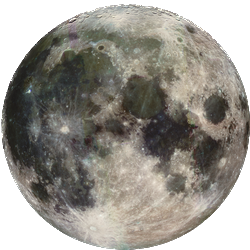
\includegraphics[width=.5cm]{../Figure/TBP/Moon.png}};
	% Text 
	\node[below, shift={(0,-0.4)}] at (MOON) {$m_2$};
	\node (b) at (B) {ماه};
	
	% Lines
	\draw[-stealth] (a) to[bend left=30] ({\r*cos(\Phi)+1},{\r*sin(\Phi)+2});
	\draw[-stealth] (b) to[bend left=-30] (MOON);
	\draw[dashed, black] (earth) -- (MOON.center);
	
	% center of mass 0.25 from earth
	\coordinate (center) at ($(earth)!0.3!(MOON)$);
	% small circle
	\draw[fill=black] (center) circle (1.5pt) node[below, shift={(0,-0.1)}] {جرم مرکز };
	
	% Calculate direction from Earth to Moon
	\pgfmathsetmacro{\xDiff}{8 - 1} % X difference between Moon and Earth
	\pgfmathsetmacro{\yDiff}{1 - 2} % Y difference between Moon and Earth
	\pgfmathsetmacro{\angle}{atan2(\yDiff,\xDiff)} % Angle of the line
	
	% Add axes at center of mass
	\draw[->, thick] (center) -- ++(\angle:2) node[above, shift={(0,0.2)}] {محور $x$};
	\draw[->, thick] (center) -- ++(\angle+90:2) node[above] {محور $y$};
	
	% add satellite with shift
	\coordinate (satellite) at ($(center)!0.5!(MOON)+(0,2)$);
	\node (satellite) at (satellite) {\faSatellite};
	
	% connect earth to satellite r1
	\draw[-stealth] (earth) -- (satellite) node[pos=0.3, above] {$\vb{r}_1$};   
	% connect moon to satellite r2
	\draw[-stealth] (MOON) -- (satellite) node[pos=0.5, above] {$\vb{r}_2$};
	% connect center of mass to satellite r
	\draw[-stealth] (center) -- (satellite) node[pos=0.5, above] {$\vb{r}$};
	% add line to show satellite is in between
	\node (c) at ($(satellite)+(1.5,0.5)$) {فضاپیما};
	\draw[-stealth] (c) to[bend left=30] (satellite);
	
\end{tikzpicture}
\caption{هندسه‌ی مسئله‌ی سه‌جسمیِ محدود در چارچوبِ چرخان}
\end{figure}



\subsection{لاگرانژ و معادلات حرکت}
با در نظر گرفتن
$G=1$
در حالت بی‌بُعد،
تابعِ لاگرانژِ جرمِ سوم در دستگاهِ چرخان برابر است با\cite{vallado2001fundamentals}
\begin{equation}\label{eq:L_crtbp}
	L=\tfrac12\bigl(\dot x^{2}+\dot y^{2}+\dot z^{2}\bigr)
	+(1-\mu)\,\frac{1}{r_{1}}+\mu\,\frac{1}{r_{2}}
	+\tfrac12\bigl(x^{2}+y^{2}\bigr),
\end{equation}
که در آن
\begin{equation}
	r_{1}=\sqrt{(x+\mu)^{2}+y^{2}+z^{2}},\qquad
	r_{2}=\sqrt{\bigl(x-1+\mu\bigr)^{2}+y^{2}+z^{2}}.
\end{equation}

با به‌کارگیری رابطه‌ی اویلر–لاگرانژ
\begin{equation*}
	\frac{\mathrm d}{\mathrm dt}\frac{\partial L}{\partial \dot q_{i}}-
	\frac{\partial L}{\partial q_{i}}=0,\qquad q_{i}\in\{x,y,z\},
\end{equation*}
معادلاتِ بی‌بُعدِ حرکتِ جرمِ سوم به دست می‌آید:
\begin{align}
	\ddot x-2\dot y &=
	x-\frac{1-\mu}{r_{1}^{3}}(x+\mu)-\frac{\mu}{r_{2}^{3}}\bigl(x-1+\mu\bigr),\\[2pt]
	\ddot y+2\dot x &=
	y-\frac{1-\mu}{r_{1}^{3}}\,y-\frac{\mu}{r_{2}^{3}}\,y,\\[2pt]
	\ddot z &= -\frac{1-\mu}{r_{1}^{3}}\,z-\frac{\mu}{r_{2}^{3}}\,z.
\end{align}
یا به نگاشتِ برداری به‌صورت زیر است.
\begin{equation}
	\ddot{\mathbf r}+2\,\boldsymbol\omega\times\dot{\mathbf r}=\nabla\Omega(\mathbf r),\qquad
	\Omega(x,y,z)=\tfrac12\bigl(x^{2}+y^{2}\bigr)+\frac{1-\mu}{r_{1}}+\frac{\mu}{r_{2}}.
\end{equation}
که در آن $\Omega$ پتانسیلِ مؤثر است و در بخش \ref{sec:lag-points} برای یافتنِ نقاطِ تعادل از شرطِ $\nabla\Omega=0$ استفاده می‌شود.
%ترم‌های کورولیس~$\pm2\,\dot{\vphantom y}$ پیامد استفاده از چارچوبِ چرخان است.


%\pgfmathsetmacro{\r}{0.8}	
%\pgfmathsetmacro{\Phi}{-160}
%\pgfmathsetmacro{\Theta}{-90}
%
%\begin{figure}[H]
%	\centering
%	\begin{tikzpicture}
%		%Grid
%		%		\draw[thin, dotted] (0,0) grid (8,8);
%		%		\foreach \i in {1,...,8}
%		%		{
%			%			\node at (\i,-2ex) {\i};	
%			%		}
%		%		\foreach \i in {1,...,8}
%		%		{
%			%			\node at (-2ex,\i) {\i};	
%			%		}
%		%		\node at (-2ex,-2ex) {0};
%		
%		% Coordinates
%		\coordinate (earth) at (1,2);
%		\coordinate (moon) at (8,1);
%		\coordinate (earth-point1) at ({\r*cos(\Theta)+1},{\r*sin(\Theta)+2});
%		\coordinate (A) at (-.5,.5);
%		\coordinate (B) at (8.5,-0.5);
%		
%		% Earth
%		\draw[thick, fill=black!30, draw=black!30
%		] (earth) circle (\r);
%		% Text
%		\node[below, shift={(0,-0.8)}] at (earth) {$m_1$};
%		\node (a) at (A) {Earth};
%		
%		% Moon
%		\node[circle, inner sep=5.5pt, fill=black!30] (MOON) at (moon) {};
%		% Text 
%		\node[below, shift={(0,-0.4)}] at (MOON) {$m_2$};
%		\node (b) at (B) {Moon};
%		
%		% Lines
%		% \draw[-latex] (earth) -- (MOON) node[pos=.55, below left] {$\vb{r}_o$};
%		% \draw[-latex] (earth) -- (earth-point1) node [pos=0.6, left] {$\vb{r}$};
%		\draw[-stealth] (a) to[bend left=30] ({\r*cos(\Phi)+1},{\r*sin(\Phi)+2});
%		\draw[-stealth] (b) to[bend left=-30] (MOON);
%		\draw[dashed, black] (earth) -- (MOON.center);
%		
%		% center of mass 0.25 from earth
%		\coordinate (center) at ($(earth)!0.3!(MOON)$);
%		% small circle
%		\draw[fill=black] (center) circle (1.5pt) node[below, shift={(0,-0.1)}] {Center of Mass};
%		% add satellite with shift
%		\coordinate (satellite) at ($(center)!0.5!(MOON)+(0,2)$);
%		% \node at ($(center)!0.5!(MOON)+(0,2)$) {\faSatellite};
%		% shift coordinate
%		\node (satellite) at (satellite) {\faSatellite};
%		
%		% connect earth to satellite r1
%		\draw[-stealth] (earth) -- (satellite) node[pos=0.5, above] {$\vb{r}_1$};   
%		% connect moon to satellite r2
%		\draw[-stealth] (MOON) -- (satellite) node[pos=0.5, above] {$\vb{r}_2$};
%		% connect center of mass to satellite r
%		\draw[-stealth] (center) -- (satellite) node[pos=0.5, above] {$\vb{r}$};
%		% add line to show satellite is in between
%		\node (c) at ($(satellite)+(1.5,0.5)$) {Satellite};
%		\draw[-stealth] (c) to[bend left=30] (satellite);
%		
%		
%		
%		
%		
%		% % Angles
%		% \pic[draw, "$\theta$", angle eccentricity=2.5, angle radius=5pt] {angle = moon--earth--earth-point1};
%		
%		% % Point
%		% \draw[fill=black] (earth) circle (1pt) node[below, shift={(0,-0.1)}] {$\mathrm{O}$};
%	\end{tikzpicture}
%	\caption{هندسه مسئله سه بدنه محدود}
%\end{figure}

%\section{نقاط لاگرانژ در مسأله‌ی سه‌جسمی محدود دایره‌ای} 
%
%
%
%\section{} نقاط تعادل (نقاط لاگرانژ $L_1$ تا $L_5$)  
%منظور از نقطه‌ی تعادل، حالتی است که جرم سوم (ذره‌ی آزمون) در دستگاه مرجع چرخان نسبت به دو جرم اصلی **ساکن** بماند. این شرایط زمانی رخ می‌دهد که سرعت و شتاب جرم سوم در دستگاه چرخان صفر شود. به‌عبارت دیگر در معادلات بالا باید $\dot{x}=\dot{y}=\dot{z}=0$ و $\ddot{x}=\ddot{y}=\ddot{z}=0$ قرار دهیم. با اعمال این شرط به معادلات لاگرانژ، مجموعه‌ای از معادلات جبری به‌دست می‌آید که مختصات نقاط تعادل (موسوم به **نقاط لاگرانژ**) را تعیین می‌کند. با قراردادن $\dot{x}=\dot{y}=0$ و $\ddot{x}=\ddot{y}=0$ در معادلات داریم:
%
%$$ 
%\begin{cases}
%	\displaystyle 0 \;=\; x \;-\; \dfrac{1-\mu}{r_1^3}(x+\mu) \;-\; \dfrac{\mu}{r_2^3}\Big(x-(1-\mu)\Big)~,  \\[2ex]
%	\displaystyle 0 \;=\; y \;-\; \dfrac{1-\mu}{r_1^3}\,y \;-\; \dfrac{\mu}{r_2^3}\,y~,  \\[1ex]
%	0 \;=\; -\,\dfrac{1-\mu}{r_1^3}\,z \;-\; \dfrac{\mu}{r_2^3}\,z~. 
%\end{cases}
%$$
%
%معادله‌ی سوم در بالا نشان می‌دهد یا باید $z=0$ باشد (نقاط تعادل همگی در صفحه‌ی حرکت هستند) یا عبارت داخل آن صفر شود که برای $z\neq0$ تنها در حالت خاصی مانند $\mu=0$ امکان‌پذیر است. بنابراین برای یافتن نقاط تعادل، حرکت جرم سوم را در همان صفحه‌ی مداری در نظر می‌گیریم ($z=0$). در این صورت $r_1$ و $r_2$ در صفحه به ترتیب $\sqrt{(x+\mu)^2+y^2}$ و $\sqrt{\big(x-(1-\mu)\big)^2+y^2}$ خواهند بود. دو معادله‌ی اول را می‌توان به صورت ساده‌تری نوشت:
%
%$$ 
%\begin{cases}
%	\displaystyle x - \dfrac{1-\mu}{r_1^3}(x+\mu) - \dfrac{\mu}{r_2^3}\Big(x-(1-\mu)\Big) = 0~,  \\[2ex]
%	\displaystyle y\,\Big[\,1 - \dfrac{1-\mu}{r_1^3} - \dfrac{\mu}{r_2^3}\Big] = 0~. 
%\end{cases}
%$$
%
%از معادله‌ی دوم نتیجه می‌شود که یا $y=0$ (نقطه‌ی تعادل روی محور $x$ واقع است) و یا پرانتز دوم صفر باشد (که منجر به رابطه‌ای بین فواصل می‌شود). بر این اساس، نقاط تعادل به دو دسته‌ی کلی تقسیم می‌شوند:
%
%- **نقاط هم‌خط (Collinear)**: این سه نقطه روی خط واصل دو جرم اصلی (محور $x$) واقع شده و بنابراین $y=0$ دارند. این نقاط را به ترتیب $L_1$، $L_2$ و $L_3$ می‌نامند.  
%- **نقاط سه‌گوش (Triangular)**: این دو نقطه در صفحه به‌صورت رئوس مثلث متساوی‌الاضلاع با دو جرم اصلی قرار می‌گیرند و دارای $y\neq0$ هستند. این دو نقطه $L_4$ و $L_5$ نام دارند.  
%
%در ادامه، هر دسته را جداگانه بررسی می‌کنیم.
%
%\section{} نقاط لاگرانژ هم‌خط ($L_1$, $L_2$, $L_3$)  
%برای نقاط واقع بر محور $x$، شرط $y=0$ را در معادلات تعادل اعمال می‌کنیم. آنگاه معادله‌ی دوم به‌طور خودکار ارضا می‌شود (زیرا $y=0$ آن را صفر می‌کند) و تنها معادله‌ی اول باقی می‌ماند:
%
%$$ 
%x - \dfrac{1-\mu}{|x+\mu|^3}(x+\mu) - \dfrac{\mu}{|x-(1-\mu)|^3}\Big(x-(1-\mu)\Big) = 0~,
%$$
%
%که در آن به علت قدرمطلق، بسته به ناحیه‌ی قرارگیری $x$، علامت عبارت‌ها مشخص می‌شود. خوشبختانه می‌توان سه ناحیه‌ی متمایز را در نظر گرفت که متناظر با سه ریشه‌ی این معادله هستند:  
%
%- **$L_1$:** بین دو جرم اصلی واقع است. در این حالت $x$ بین $-\mu$ و $1-\mu$ قرار دارد (بین موقعیت‌های جرم اول و جرم دوم). برای $L_1$ فاصله‌ی آن از جرم دوم را با $d_1$ نشان می‌دهیم (پس $x = (1-\mu) - d_1$). این فاصله را می‌توان با حل معادله‌ی بالا به‌دست آورد. معادله‌ی تعادل در این ناحیه را می‌توان پس از ساده‌سازی به صورت یک معادله‌ی درجه پنج (در $x$ یا $d_1$) نوشت که جواب تحلیلی ساده‌ای ندارد و معمولاً به روش عددی (مثلاً روش نیوتن) حل می‌شود. با این وجود، برای $\mu$های کوچک (مثلاً سیستمی مانند خورشید-زمین یا زمین-ماه) می‌توان تخمین خوبی به‌دست آورد. اگر $\mu \ll 1$ باشد (جرم دوم بسیار کوچک‌تر از جرم اول)، آنگاه $L_1$ بسیار نزدیک به جرم دوم خواهد بود و فاصله‌ی آن از جرم دوم (در واحد فاصله‌ی دو جرم اصلی) تقریباً برابر **شعاع کره‌ی هیل** جرم دوم است. شعاع هیل تقریباً $r_h \approx (\mu/3)^{1/3}$ است. بنابراین می‌توان نوشت: 
%
%$$d_1 \approx \Big(\dfrac{\mu}{3}\Big)^{1/3},$$ 
%
%و در نتیجه مختصات $L_1$ تقریباً برابر است با: 
%
%$$x_{L_1} \approx (1-\mu) - (\mu/3)^{1/3}, \qquad y_{L_1}=0.$$ 
%
%(توجه شود که برای دقت بیشتر، در صورت نیاز باید اثر $\mu$ را در قسمت $(1-\mu)$ نیز لحاظ کرد.) این فرمول یک تخمین از موقعیت $L_1$ است. در عمل حل عددی دقیق معادله، مقدار دقیق‌تری برای $x_{L_1}$ به‌دست می‌دهد. این نقطه جایی است که نیروی گرانش دو جرم (یکی کشنده به چپ و دیگری به راست) و نیروی گریز از مرکز دقیقا همدیگر را خنثی می‌کنند. 
%
%- **$L_2$:** بیرون جرم دوم (کوچک) و در امتداد همان محور قرار دارد. این نقطه در سمت راست جرم دوم واقع است ($x > 1-\mu$) و جرم دوم بین آن و جرم اول قرار می‌گیرد. اگر فاصله‌ی $L_2$ از جرم دوم را $d_2$ بگیریم ($x = (1-\mu) + d_2$)، معادله‌ی تعادل در این ناحیه نیز پس از ساده‌سازی یک معادله‌ی درجه پنج برای $d_2$ خواهد بود که باید عددی حل شود. برای $\mu$ کوچک (جرم دوم خیلی کوچک‌تر)، این فاصله نیز تقریباً برابر $(\mu/3)^{1/3}$ به‌دست می‌آید. یعنی: 
%
%$$d_2 \approx \Big(\dfrac{\mu}{3}\Big)^{1/3},$$ 
%
%و بنابراین: 
%
%$$x_{L_2} \approx (1-\mu) + (\mu/3)^{1/3}, \qquad y_{L_2}=0.$$ 
%
%این نقطه در بیرون مدار جرم دوم قرار دارد و تعادل نیروها در آن به این صورت است که نیروی گریز از مرکز به سمت بیرون توسط مجموع نیروی گرانشی دو جرم (هر دو به سمت داخل) بالانس می‌شود. 
%
%- **$L_3$:** بیرون جرم اول (بزرگ) و در امتداد خط محور $x$ در سمت مقابل جرم دوم واقع است ($x < -\mu$). این نقطه در سوی دیگر جرم بزرگ‌تر قرار دارد به‌طوری که جرم اول بین $L_3$ و جرم دوم است. برای $L_3$ نیز معادله‌ی تعادل به روش عددی حل می‌شود؛ و در حد $\mu \ll 1$ (جرم دوم بسیار کوچک)، موقعیت آن اندکی فراتر از مدار جرم اول (جرم بزرگ) است. می‌توان نشان داد برای $\mu$های بسیار کوچک: 
%
%$$x_{L_3} \approx -\,1 - \dfrac{5}{12}\,\mu, \qquad y_{L_3}=0,$$ 
%
%که نشان می‌دهد $L_3$ تقریباً به اندازه‌ی فاصله‌ی دو جرم اصلی دورتر از جرم اول است (حد $\mu \to 0$ منجر به $x=-1$ می‌شود که درست در سمت مقابل جرم دوم و هم‌فاصله با آن است) و با در نظر گرفتن جرم کوچک دوم، اندکی بیش از آن (چند صدم درصد بسته به مقدار $\mu$) فاصله می‌گیرد. به بیان دیگر، گرانش جرم دوم (هرچند کوچک) باعث می‌شود برای حفظ تعادل، جرم سومِ واقع در $L_3$ کمی به جرم بزرگ‌تر نزدیک‌تر شود تا نیروی گریز از مرکز کمتر شده و با کاهش کمی در فاصله، گرانش جرم بزرگ افزایش یابد و تعادل برقرار گردد.  
%
%معمولاً معادله‌ی دقیق مربوط به $L_1$, $L_2$ و $L_3$ را به صورت یک چندجمله‌ای درجه ۵ نسبت به متغیری کمکی بیان می‌کنند (که به **معادله‌ی کوئینتیک لاگرانژ** مشهور است) و سپس آن را با تقریب یا روش‌های عددی حل می‌نمایند. به عنوان مثال، در مراجع کلاسیک نشان داده می‌شود که اگر $\rho = x + \mu$ فاصله‌ی مرکز جرم تا نقطه‌ی تعادل در یک جهت در نظر گرفته شود، معادله‌ی درجه پنج در $\rho$ قابل بیان است. اما در کاربردهای عملی، استفاده از روش‌های عددی سریع‌تر به جواب منجر می‌شود. 
%
%\section{} نقاط لاگرانژ سه‌گوش ($L_4$, $L_5$)  
%دو نقطه‌ی تعادل دیگر در صفحه‌ی مدار به‌صورتی قرار می‌گیرند که همراه با دو جرم اصلی تشکیل یک مثلث متساوی‌الاضلاع بدهند. در چنین آرایشی، جرم سوم می‌تواند در حالت تعادل نسبی (هم‌دوران با دو جرم دیگر) باقی بماند. برای این نقاط، واضح است که $y \neq 0$ خواهد بود. بنابراین در معادلات تعادل باید قسمت داخل کروشه (که در معادله‌ی تعادل $y$ ظاهر شد) صفر گردد:
%
%$$1 - \dfrac{1-\mu}{r_1^3} - \dfrac{\mu}{r_2^3} = 0.$$
%
%این رابطه همراه با معادله‌ی تعادل در $x$ باید همزمان ارضا شوند. از آنجا که مثلث متساوی‌الاضلاع است، فاصله‌ی جرم سوم از هر دو جرم اصلی برابر است ($r_1 = r_2$). با توجه به واحد طول نرمال‌شده (فاصله‌ی بین دو جرم اصلی برابر ۱)، این فاصله باید برابر با ۱ (طول ضلع مثلث) باشد. لذا $r_1 = r_2 = 1$. در این صورت، رابطه‌ی فوق به سادگی $1 - (1-\mu) - \mu = 0$ خواهد بود که برقرار است. با استفاده از هندسه‌ی مثلث متساوی‌الاضلاع در دستگاه مختصات تعریف‌شده می‌توان مختصات دقیق $L_4$ و $L_5$ را به‌دست آورد. اگر ضلع پایینی مثلث روی محور $x$ باشد (جرم‌ها روی محور $x$ قرار دارند) و جرم سوم رأس مثلث باشد، آنگاه مختصات آن عبارت‌اند از:
%
%$$ 
%x_{L_4} \;=\; x_{L_5} \;=\; \dfrac{1}{2} - \mu~, \qquad 
%y_{L_4} \;=\; +\dfrac{\sqrt{3}}{2}~, \qquad 
%y_{L_5} \;=\; -\dfrac{\sqrt{3}}{2}~.
%$$
%
%به بیان دیگر، در دستگاه باریسنتر چرخان، هر دوی $L_4$ و $L_5$ به اندازه‌ی نیمی از فاصله‌ی دو جرم روی محور $x$ از مرکز جرم فاصله دارند (کمی جابه‌جا‌شده به سمت جرم بزرگ‌تر به اندازه‌ی $\mu$) و مؤلفه‌ی عمودی (محور $y$) آن‌ها برابر $\pm\dfrac{\sqrt{3}}{2}$ است که نشان‌دهنده‌ی زاویه‌ی $60^\circ$ نسبت به محور $x$ می‌باشد. این دو نقطه، در صورت کافی‌بودن نسبت جرم‌ها (بزرگ‌تر بودن قابل توجه جرم اول نسبت به جرم دوم؛ معمولاً $\dfrac{m_1}{m_2} > 24.96$ شرط پایداری است)، **نقاط تعادل پایدار** هستند. به عنوان مثال سیاره‌ی مشتری تعداد زیادی سیارک‌های تروجان در نقاط $L_4$ و $L_5$ خود نسبت به خورشید دارد. در مقابل، سه نقطه‌ی هم‌خط ($L_1,L_2,L_3$) پایداری ذاتی ندارند و اجسام در آن‌ها بدون تصحیح مداری معمولا از نقطه‌ی تعادل دور می‌شوند، با این حال برای تحقیقات فضایی (مانند رصدخانه‌ها یا رله‌های مخابراتی) محبوب‌اند زیرا مدارهای هاله‌ای یا لیساژور حول این نقاط با صرف انرژی اندک قابل حفظ هستند.
%
%\section{} نمونه: نقاط لاگرانژ در سیستم زمین-ماه  
%برای سیستم زمین-ماه مقدار $\mu \approx 0.01215$ است (نسبت جرم ماه به مجموع جرم زمین و ماه). در این سیستم با اعمال روابط به‌دست‌آمده می‌توان موقعیت عددی هر پنج نقطه‌ی لاگرانژ را محاسبه کرد. جدول زیر مختصات بی‌بعد (بر حسب فاصله‌ی زمین-ماه به عنوان واحد طول) این نقاط را در دستگاه مختصات تعریف‌شده‌ی باریسنتر (مرکز جرم در مبدأ، زمین در مختصات $(-\mu,0)$ و ماه در $(1-\mu,0)$) نشان می‌دهد. لازم به ذکر است که در این مقیاس، مختصات زمین تقریباً $(-0.01215,\;0)$ و ماه $(0.98785,\;0)$ می‌باشد. همان‌طور که مشاهده می‌شود، $L_1$ حدوداً در 84\% فاصله‌ی زمین-ماه (از سمت زمین) واقع شده و $L_2$ کمی بیرون مدار ماه قرار دارد. نقطه‌ی $L_3$ اندکی آن‌سوی مدار زمین (در جهت مخالف ماه) است. نقاط $L_4$ و $L_5$ نیز به‌ترتیب در بالا و پایین صفحه (در زاویه‌ی $60^\circ$) و تقریباً در فاصله‌ی مساوی از زمین و ماه قرار گرفته‌اند.
%
%| نقطه‌ی لاگرانژ | $x$ (بی‌بعد)     | $y$ (بی‌بعد)    |
%%| -------------- | -------------- | -------------- |
%%| $L_1$          | $+0.83692$     | $0$            |
%%| $L_2$          | $+1.15568$     | $0$            |
%%| $L_3$          | $-1.00506$     | $0$            |
%%| $L_4$          | $+0.48785$     | $+0.86603$     |
%%| $L_5$          | $+0.48785$     | $-0.86603$     |
%
%
%\begin{table}[H]
%	\centering
%	\caption{مقادیر عددی برای مسئله سه‌جسمی محدود (سیستم زمین-ماه)}
%\begin{tabular}{|c|c|c|}
%	\hline
%	\text{نقطه‌ی لاگرانژ} & \(x\) \, (\text{بی‌بعد}) & \(y\) \, (\text{بی‌بعد}) \\
%	\hline
%	$L_1$ & $+0.83692$ & $0$ \\
%	$L_2$ & $+1.15568$ & $0$ \\
%	$L_3$ & $-1.00506$ & $0$ \\
%	$L_4$ &$ +0.48785$ & $+0.86603$ \\
%	$L_5$ & $+0.48785$ & $-0.86603$ \\
%	\hline  
%\end{tabular}
%\end{table}
%
%
%
%
%
%
%
%
%
%\begin{figure}
%	\centering
%	\begin{tikzpicture}
%		% Define radius of the orbit
%		\def\orbitRadius{4cm}
%		
%		% Draw the orbit circle with arrows
%		\draw[-{Stealth[length=3mm]}, thick] (12:\orbitRadius) arc (12:170:\orbitRadius);
%		\draw[-{Stealth[length=3mm]}, thick] (180:\orbitRadius) arc (180:355:\orbitRadius);
%		
%		% Position for Earth (center)
%		\node[inner sep=0pt] (Earth) at (0,0) {
\includegraphics[width=1.8cm]{../Figure/TBP/Earth.png}};
%		\node[text=black] at (0,-1.3) {Earth};
%		
%		% Position for Moon (on the right side of the orbit)
%		\node[inner sep=0pt] (Moon) at (0.95*\orbitRadius,0) {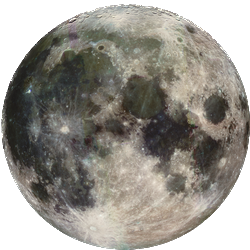
\includegraphics[width=0.6cm]{../Figure/TBP/Moon.png}};
%		\node[text=black] at (\orbitRadius,0.75) {Moon};
%		
%		% Lagrangian points
%		\coordinate (L1) at (0.8*\orbitRadius,0);
%		\coordinate (L2) at (1.2*\orbitRadius,0);
%		\coordinate (L3) at (-1*\orbitRadius,0);
%		\coordinate (L4) at (60:\orbitRadius);
%		\coordinate (L5) at (300:\orbitRadius);
%		
%		% Draw Lagrangian points as red circles
%		\foreach \point in {L1,L2,L3,L4,L5} {
%			\fill[red] (\point) circle (0.1cm);
%		}
%		
%		% Connect Lagrangian points with dashed green lines
%		\draw[dashed, blue, thick] (Earth) -- (L1);
%		\draw[dashed, blue, thick] (Moon) -- (L1);
%		\draw[dashed, blue, thick] (Moon) -- (L2);
%		\draw[dashed, blue, thick] (Earth) -- (L3);
%		\draw[dashed, blue, thick] (Earth) -- (L4);
%		\draw[dashed, blue, thick] (Moon) -- (L4);
%		\draw[dashed, blue, thick] (Earth) -- (L5);
%		\draw[dashed, blue, thick] (Moon) -- (L5);
%		
%		% Labels for the Lagrangian points
%		\node at ($(L1) + (0,0.5)$) {$L_1$};
%		\node at ($(L2) + (0,0.5)$) {$L_2$};
%		\node at ($(L3) + (0,0.5)$) {$L_3$};
%		\node at ($(L4) + (0.5,0.3)$) {$L_4$};
%		\node at ($(L5) + (0.5,-0.3)$) {$L_5$};
%	\end{tikzpicture}
%	\caption{نقاط لاگرانژ}
%\end{figure}
%
%
%
%
%
%
%
%
%
%
%
%در جدول بالا علامت مثبت/منفی $x$ نشان‌دهنده‌ی موقعیت نسبت به مرکز جرم (مبدأ مختصات) روی محور زمین-ماه است (مثبت به سمت ماه و منفی به سمت زمین) و محور $y$ عمود بر آن صفحه‌ی مداری در جهت چرخش سیستم تعریف شده است. مقادیر عددی ارائه‌شده نشان می‌دهند که در منظومه‌ی زمین-ماه، $L_1$ تقریباً در فاصله‌ی $0.84$ برابر فاصله‌ی زمین-ماه از زمین قرار دارد (یعنی فاصله‌ی آن از ماه حدود $0.16$ برابر فاصله‌ی زمین-ماه است). به طور مشابه $L_2$ حدود $1.156$ برابر فاصله‌ی زمین-ماه از زمین فاصله دارد (حدود $0.156$ برابر فاصله‌ی زمین-ماه آن‌سوی مدار ماه). نقطه $L_3$ تقریباً در فاصله‌ای برابر با فاصله‌ی زمین-ماه در سمت مقابل (پشت زمین نسبت به ماه) قرار گرفته است. نقاط $L_4$ و $L_5$ نیز تقریباً در مختصات $(0.488,\;\pm0.866)$ واقع شده‌اند که نشان‌دهنده‌ی تشکیل مثلث متساوی‌الاضلاع با زمین و ماه می‌باشد. این مقادیر و تحلیلات تأیید می‌کنند که روابط تحلیلی به‌دست‌آمده برای معادلات لاگرانژ و نقاط تعادل، به‌خوبی می‌توانند برای توصیف وضعیت‌های پایدار و ناپایدار یک جرم کوچک در میدان گرانشی دو جرم آسمانی به‌کار روند. 
%
%**مراجع:**  
%1. Richard H. Battin, *An Introduction to the Mathematics and Methods of Astrodynamics*, Revised Edition, AIAA Education Series, Eq.(1) for Lagrange’s quintic equation. (معادله درجه پنج لاگرانژ برای محاسبه نقاط $L_1, L_2, L_3$)









%--------------------------------------------------------------
\section{نقاط تعادلِ لاگرانژ}\label{sec:lag-points}

نقطه‌ی تعادل مکانی است که در چارچوبِ چرخان، جرمِ سوم بی‌حرکت بماند. این شرایط با صفرشدن مؤلفه‌های سرعت و شتاب به‌دست می‌آید؛ ازاین‌رو در معادلاتِ بالا قرار می‌دهیم $\dot x=\dot y=\dot z=\ddot x=\ddot y=\ddot z=0$. در نتیجه دستگاهِ جبریِ زیر برای مختصاتِ نقطه‌ی تعادل حاصل می‌شود:
\begin{align}
	0 &= x-\frac{1-\mu}{r_{1}^{3}}(x+\mu)-\frac{\mu}{r_{2}^{3}}\bigl(x-1+\mu\bigr),\\
	0 &= y\Bigl[1-\frac{1-\mu}{r_{1}^{3}}-\frac{\mu}{r_{2}^{3}}\Bigr],\\
	0 &= -\frac{1-\mu}{r_{1}^{3}}\,z-\frac{\mu}{r_{2}^{3}}\,z.
\end{align}
معادله‌ی سوم نشان می‌دهد برای حالت عمومی باید $z=0$ باشد؛ بنابراین نقاطِ تعادل همگی در صفحه‌ی مدار قرار می‌گیرند.

\subsubsection{دسته‌بندی کلی}
\begin{enumerate}
	\item {نقاطِ هم‌خط (\lr{Collinear}).} سه نقطه‌ی $L_{1}$، $L_{2}$ و $L_{3}$ روی خط واصلِ دو جرم قرار دارند و لذا $y=0$ است.
	\item {نقاطِ سه‌گوش (\lr{Triangular}).} دو نقطه‌ی $L_{4}$ و $L_{5}$ رأس‌های مثلثِ متساوی‌الاضلاع با دو جرمِ اصلی را تشکیل می‌دهند و در آن‌ها $y\ne0$.
\end{enumerate}



\begin{figure}[H]
	\centering
	\begin{tikzpicture}
		% Define radius of the orbit
		\def\orbitRadius{4cm}
		
		% Draw the orbit circle with arrows
		\draw[-{Stealth[length=3mm]}, thick] (12:\orbitRadius) arc (12:170:\orbitRadius);
		\draw[-{Stealth[length=3mm]}, thick] (180:\orbitRadius) arc (180:355:\orbitRadius);
		
		% Position for Earth (center)
		\node[inner sep=0pt] (Earth) at (0,0) {
\includegraphics[width=1.8cm]{../Figure/TBP/Earth.png}};
		\node[text=black] at (0,-1.3) {Earth};
		
		% Position for Moon (on the right side of the orbit)
		\node[inner sep=0pt] (Moon) at (0.95*\orbitRadius,0) {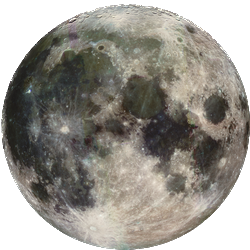
\includegraphics[width=0.6cm]{../Figure/TBP/Moon.png}};
		\node[text=black] at (\orbitRadius,0.75) {Moon};
		
		% Lagrangian points
		\coordinate (L1) at (0.8*\orbitRadius,0);
		\coordinate (L2) at (1.2*\orbitRadius,0);
		\coordinate (L3) at (-1*\orbitRadius,0);
		\coordinate (L4) at (60:\orbitRadius);
		\coordinate (L5) at (300:\orbitRadius);
		
		% Draw Lagrangian points as red circles
		\foreach \point in {L1,L2,L3,L4,L5} {
			\fill[red] (\point) circle (0.1cm);
		}
		
		% Connect Lagrangian points with dashed green lines
		\draw[dashed, blue, thick] (Earth) -- (L1);
		\draw[dashed, blue, thick] (Moon) -- (L1);
		\draw[dashed, blue, thick] (Moon) -- (L2);
		\draw[dashed, blue, thick] (Earth) -- (L3);
		\draw[dashed, blue, thick] (Earth) -- (L4);
		\draw[dashed, blue, thick] (Moon) -- (L4);
		\draw[dashed, blue, thick] (Earth) -- (L5);
		\draw[dashed, blue, thick] (Moon) -- (L5);
		
		% Labels for the Lagrangian points
		\node at ($(L1) + (0,0.5)$) {$L_1$};
		\node at ($(L2) + (0,0.5)$) {$L_2$};
		\node at ($(L3) + (0,0.5)$) {$L_3$};
		\node at ($(L4) + (0.5,0.3)$) {$L_4$};
		\node at ($(L5) + (0.5,-0.3)$) {$L_5$};
	\end{tikzpicture}
	\caption{نقاط لاگرانژ}
\end{figure}



%--------------------------------------------------------------
\subsubsection{نقاطِ هم‌خط \texorpdfstring{$(L_{1},L_{2},L_{3})$}{(L1,L2,L3)}}\label{subsec:collinear}

با اعمال $y=0$، تنها معادله‌ی زیر باقی می‌ماند
\begin{equation}\label{eq:collinear_eq}
	x-\frac{1-\mu}{|x+\mu|^{3}}(x+\mu)-\frac{\mu}{|x-1+\mu|^{3}}\bigl(x-1+\mu\bigr)=0.
\end{equation}
این معادله در سه ناحیه‌ی مجزا—بین دو جرم، بیرونِ جرمِ کوچک و بیرونِ جرمِ بزرگ—دارای یک ریشه است که به‌ترتیب نقاطِ $L_{1}$، $L_{2}$ و $L_{3}$ را تعیین می‌کند.

برای $\mu\ll1$ (همچون سامانه‌ی خورشید–زمین یا زمین–ماه) می‌توان تقریب‌های شناخته‌شده را نوشت:
\begin{align*}
	x_{L_{1}} &\simeq (1-\mu)-\bigl(\tfrac{\mu}{3}\bigr)^{1/3},\\
	x_{L_{2}} &\simeq (1-\mu)+\bigl(\tfrac{\mu}{3}\bigr)^{1/3},\\
	x_{L_{3}} &\simeq -1-\tfrac{5}{12}\,\mu; \qquad y_{L_{i}}=0.
\end{align*}
در عمل، ریشه‌ی دقیقِ معادله‌ی \eqref{eq:collinear_eq} با یک روشِ عددی (نیوتن–رافسون) محاسبه می‌شود.

%--------------------------------------------------------------
\subsubsection{نقاطِ سه‌گوش \texorpdfstring{$(L_{4},L_{5})$}{(L4,L5)}}\label{subsec:triangular}

در این نقاط $r_{1}=r_{2}=1$ و شرطِ
\(1-(1-\mu)/r_{1}^{3}-\mu/r_{2}^{3}=0\)\, به طور طبیعی برقرار است. مختصات به سادگی عبارت‌اند از
\begin{equation}
	x_{L_{4}}=x_{L_{5}}=\tfrac12-\mu,\qquad
	y_{L_{4}}=+\tfrac{\sqrt3}{2},\qquad
	y_{L_{5}}=-\tfrac{\sqrt3}{2}.
\end{equation}
پایداری این نقاط مستلزم نسبتِ جرمِ کافی است؛ شرطِ کلاسیک~$m_{1}/m_{2}>24.96$ در سامانه‌های خورشید–سیاره یا زمین–ماه به خوبی برقرار است و سببِ وجودِ خانواده‌ی سیارک‌های تروجان حول $L_{4}$ و $L_{5}$ می‌شود. در مقابل، نقاطِ هم‌خط ناپایدارند و معمولاً مأموریت‌های فضایی روی مدارهای هاله‌ای یا لیساژور در پیرامونِ آن‌ها قرار می‌گیرند.

%--------------------------------------------------------------
%\subsubsection{مثال: سامانه‌ی زمین–ماه}\label{subsec:earth-moon}

برای سامانه‌ی زمین–ماه، $\mu\simeq0.01215$ است. جدولِ زیر مختصاتِ بی‌بُعدِ هر پنج نقطه را نشان می‌دهد (واحدِ طول: فاصله‌ی زمین–ماه). موقعیتِ زمین در $(-\mu,0)$ و ماه در $(1-\mu,0)$ است.

\begin{table}[H]
	\centering
	\caption{مقادیر عددی نقاط لاگرانژ برای مسئله سه‌جسمی محدود سیستم زمین-ماه}
	\begin{tabular}{|c|c|c|}
		\hline
		\text{نقطه‌ی لاگرانژ} & \(x\) \, (\text{بی‌بعد}) & \(y\) \, (\text{بی‌بعد}) \\
		\hline
		$L_1$ & $+0.83692$ & $0$ \\
		$L_2$ & $+1.15568$ & $0$ \\
		$L_3$ & $-1.00506$ & $0$ \\
		$L_4$ &$ +0.48785$ & $+0.86603$ \\
		$L_5$ & $+0.48785$ & $-0.86603$ \\
		\hline  
	\end{tabular}
\end{table}











%\begin{table}[H]
%	\centering
%	\caption{مختصاتِ نقاطِ لاگرانژ برای سامانه‌ی زمین–ماه (مقیاسِ بی‌بُعد)}\label{tab:lagrange_earth_moon}
%	\begin{tabular}{ccc}
%		\toprule
%		\textbf{نقطه} & $x$ & $y$\\
%		\midrule
%		$L_{1}$ & $+0.83692$ & $0$\\
%		$L_{2}$ & $+1.15568$ & $0$\\
%		$L_{3}$ & $-1.00506$ & $0$\\
%		$L_{4}$ & $+0.48785$ & $+0.86603$\\
%		$L_{5}$ & $+0.48785$ & $-0.86603$\\
%		\bottomrule
%	\end{tabular}
%\end{table}
%
%\begin{figure}[H]
%	\centering
%	\begin{tikzpicture}[scale=1]
%		% orbit radius
%		\def\R{4cm}
%		
%		% orbit circle (arrowed)
%		\draw[-{Stealth[length=3mm]},thick] (12:\R) arc (12:170:\R);
%		\draw[-{Stealth[length=3mm]},thick] (180:\R) arc (180:355:\R);
%		
%		% Earth & Moon
%		\node[inner sep=0pt] (Earth) at (0,0)
%		{
\includegraphics[width=1.8cm]{../Figure/TBP/Earth.png}};
%		\node[below=3pt of Earth] {Earth};
%		
%		\node[inner sep=0pt] (Moon) at (0.95*\R,0)
%		{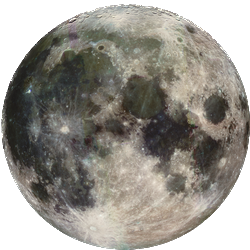
\includegraphics[width=0.6cm]{../Figure/TBP/Moon.png}};
%		\node[above right=6pt and -7pt of Moon] {Moon};
%		
%		% Lagrange coordinates
%		\coordinate (L1) at (0.8*\R,0);
%		\coordinate (L2) at (1.2*\R,0);
%		\coordinate (L3) at (-1*\R,0);
%		\coordinate (L4) at (60:\R);
%		\coordinate (L5) at (300:\R);
%		
%		% draw points
%		\foreach \P in {L1,L2,L3,L4,L5}
%		\fill[red] (\P) circle (2pt);
%		
%		% dashed helpers
%		\foreach \pair in {Earth/L1, Moon/L1, Moon/L2, Earth/L3, Earth/L4,
%			Moon/L4, Earth/L5, Moon/L5}
%		{\draw[dashed,blue] (\pair);
%		}
%		
%		% labels
%		\node[above=3pt] at (L1) {$L_1$};
%		\node[above=3pt] at (L2) {$L_2$};
%		\node[above left=2pt] at (L3) {$L_3$};
%		\node[right=4pt] at (L4) {$L_4$};
%		\node[right=4pt] at (L5) {$L_5$};
%	\end{tikzpicture}
%	\caption{جایگاه نقاطِ لاگرانژ در سامانه‌ی زمین–ماه (طرح شماتیک).}
%\end{figure}

%--------------------------------------------------------------
\noindent
این نتایج نشان می‌دهد که $L_{1}$ در حدودِ $0.84$ فاصله‌ی زمین–ماه از زمین قرار دارد (فاصله‌ی آن تا ماه در حدود $0.16$ واحد طول است) و $L_{2}$ بیرونِ مدارِ ماه است. نقطه‌ی $L_{3}$ تقریباً یک واحدِ طول در سوی مقابلِ ماه نسبت به زمین قرار دارد. دو نقطه‌ی $L_{4}$ و $L_{5}$ در مختصات $(0.488,\pm0.866)$ قرار گرفته و با زمین و ماه مثلثِ متساوی‌الاضلاع می‌سازند.
